% \documentclass[twoside,twocolumn]{article}
\documentclass{article}

\usepackage{blindtext} % Package to generate dummy text throughout this template 

% \usepackage[sc]{mathpazo}
\usepackage{mathptmx}
\usepackage[T1]{fontenc} % Use 8-bit encoding that has 256 glyphs
\linespread{1.05} % Line spacing - Palatino needs more space between lines
\usepackage{microtype} % Slightly tweak font spacing for aesthetics

\usepackage[english]{babel} % Language hyphenation and typographical rules

\usepackage[hmarginratio=1:1,top=32mm,columnsep=20pt]{geometry} % Document margins
\usepackage[hang, small,labelfont=bf,up,textfont=it,up]{caption} % Custom captions under/above floats in tables or figures
\usepackage{booktabs} % Horizontal rules in tables

\usepackage{lettrine} % The lettrine is the first enlarged letter at the beginning of the text

\usepackage{enumitem} % Customized lists
\setlist[itemize]{noitemsep} % Make itemize lists more compact

\usepackage{abstract} % Allows abstract customization
\renewcommand{\abstractnamefont}{\normalfont\bfseries} % Set the "Abstract" text to bold
\renewcommand{\abstracttextfont}{\normalfont\small\itshape} % Set the abstract itself to small italic text

\usepackage{titlesec} % Allows customization of titles
\renewcommand\thesection{\Roman{section}} % Roman numerals for the sections
\renewcommand\thesubsection{\roman{subsection}} % roman numerals for subsections
\titleformat{\section}[block]{\large\scshape\centering}{\thesection.}{1em}{} % Change the look of the section titles
\titleformat{\subsection}[block]{\large}{\thesubsection.}{1em}{} % Change the look of the section titles

\usepackage{fancyhdr} % Headers and footers
\pagestyle{fancy} % All pages have headers and footers
\fancyhead{} % Blank out the default header
\fancyfoot{} % Blank out the default footer
\fancyhead[C]{Running title $\bullet$ May 2016 $\bullet$ Vol. XXI, No. 1} % Custom header text
\fancyfoot[RO,LE]{\thepage} % Custom footer text

\usepackage{titling} % Customizing the title section

\usepackage{hyperref} % For hyperlinks in the PDF
\usepackage{graphicx}
\usepackage{amsmath}
%----------------------------------------------------------------------------------------
%	TITLE SECTION
%----------------------------------------------------------------------------------------

\setlength{\droptitle}{-4\baselineskip} % Move the title up

\pretitle{\begin{center}\Huge\bfseries} % Article title formatting
\posttitle{\end{center}} % Article title closing formatting
\title{Sliding Mode Control of a Quad-Copter for Autonomous Trajectory Tracking} % Article title
\author{%
\textsc{Daniel Wood, Majura Selekwa}\thanks{A thank you or further information} \\begin{equation}1ex] % Your name
\normalsize North Dakota State University \\ % Your institution
\normalsize \href{mailto:daniel.wood@ndsu.edu}{daniel.wood@ndsu.edu} % Your email address
%\and % Uncomment if 2 authors are required, duplicate these 4 lines if more
%\textsc{Jane Smith}\thanks{Corresponding author} \\begin{equation}1ex] % Second author's name
%\normalsize University of Utah \\ % Second author's institution
%\normalsize \href{mailto:jane@smith.com}{jane@smith.com} % Second author's email address
}
\date{\today} % Leave empty to omit a date
\renewcommand{\maketitlehookd}{%
\begin{abstract}
\noindent Unmanned air vehicles or drones have become ubiquitous in our daily lives; they are deployed in performing many tasks from dangerous military missions to simple recreation activities. One air vehicle that has become very popular is the quad-copter driven by four vertical and parallel propellers. Today quad-copters are deployed in many video recording and remote monitoring applications everywhere in the world. One area of interest for quad-copters has been in farming operations; these vehicles are used in farming operations for not only aerial monitoring of soil nitrogen levels but many other farm monitoring operations. One common aspect of most quad-copters is that they are teleoperated by the user, i.e., most of them are not yet fully autonomous. There must be a remote pilot who is connected to the quad-copter by a video link so that he/she can control the maneuver of the vehicle along the intended path. This paper intends to show that a quad-copter can be programmed to run autonomously along a predetermined trajectory by using sliding mode control strategy. Since trajectories in most farms are clearly well known in advance, they can be programmed into the controller for the quad-copter to autonomously track. The design process involves using the intended trajectory to define the 3-D sliding surface and then letting the quad-copter controller switch about that surface while keeping the vehicle in the target trajectory. The workspace is defined as a 3-D space where the sliding surface is defined by fitting weighted spline functions on the coordinates of the intended trajectory to define the stable sliding surface whose stability lever increases as the vehicle moves towards the target point. Preliminary results compare the trajectories followed by the quad-copter and the intended trajectories by using the mean square deviation. As would be expected, the performance depends heavily on the speed of the quad-copter; higher speeds on sharp curvature are associated with large tracking errors copmpared to low speeds on similar curvatures, while the performance on straight line paths was considerably good. This is  most likely due to the switching speed, as it is shown that higher speeds are associated with higher switching speeds also. The future work intends to study if parameterizing the 3-D splines using speed and time can improve the tracking performance where the switching rate will be made to be proportional to the number of spline functions that define the trajectory irrespective of the speed of the quad-copter. 
\end{abstract}
}

%----------------------------------------------------------------------------------------

\begin{document}

% Print the title
\maketitle

%----------------------------------------------------------------------------------------
%	ARTICLE CONTENTS
%----------------------------------------------------------------------------------------

\section{Introduction}

\lettrine[nindent=0em,lines=3]{T} he work of this paper focuses not on simplifying the dynamics to the point where nonlinearites are neglected. But to include the full non-linear dynamics of the system, while using a variable switching tecnique referred to as sliding mode control in 3D with the purpose of autonomous trajectory tracking. This is achieved by first taking a Euler/Lagrange approach to determine the equations of motion.

\begin{figure}
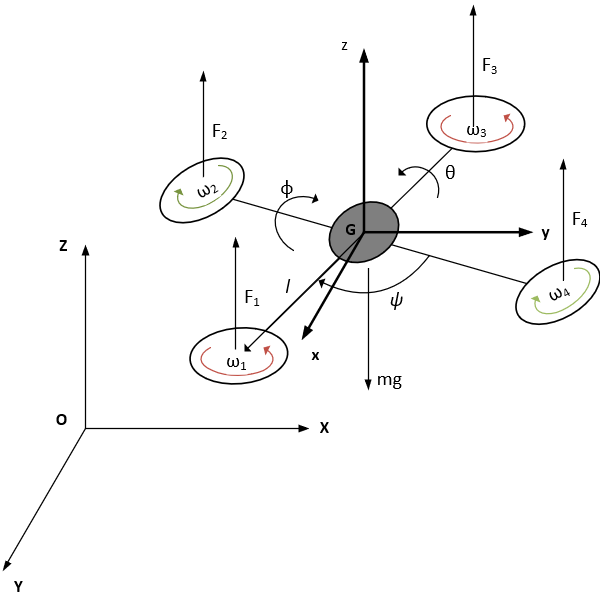
\includegraphics[scale = 0.5]{drone_diag.png}
\caption{Free Body Diagram of Quadcopter}
\end{figure}

\begin{equation}
x=[\begin{array}{cccccc}
X_{G} & Y_{G} & Z_{G} & \psi & \theta & \phi\end{array}]
\end{equation}
where $X_{G},Y_{G},Z_{G}$ are the global position of the quadcopter center of mass, and $\psi,\theta,\phi$ are the Euler angles of each axis.

This state vector will be defined in terms of generalized coordinates for the remainder of the analysis:

\begin{equation}
\begin{split}
q &= [\begin{array}{cccccc}
X_{G} & Y_{G} & Z_{G} & \psi & \theta & \phi\end{array}] \\
&= [\begin{array}{cccccc}
q_{1} & q_{2} & q_{3} & q_{4} & q_{5} & q_{6}\end{array}]
\end{split}
\end{equation}

The dynamics of the body in the inertial frame is found through Euler-Lagrange approach, with the Kinetic Energy defined as:

\begin{equation}
T(q)=\frac{1}{2}\dot{q}^{T}M(q)\dot{q}
\end{equation}

where M(q) is defined as:

\begin{equation}
M(q)=J_{v}(q)^{T}m_{rr}J_{v}(q)+J_{w}(q)^{T}m_{\theta\theta}J_{w}(q)
\end{equation}

with:

\begin{equation}
J_{v}(q)=\left[\begin{array}{cccccc}
\frac{\partial q_{1}}{\partial q_{1}} & \frac{\partial q_{1}}{\partial q_{2}} & \frac{\partial q_{1}}{\partial q_{3}} & 0 & 0 & 0\\
\frac{\partial q_{2}}{\partial q_{1}} & \frac{\partial q_{2}}{\partial q_{2}} & \frac{\partial q_{2}}{\partial q_{3}} & 0 & 0 & 0\\
\frac{\partial q_{3}}{\partial q_{1}} & \frac{\partial q_{3}}{\partial q_{1}} & \frac{\partial q_{3}}{\partial q_{1}} & 0 & 0 & 0
\end{array}\right]
\end{equation}

\begin{equation}
J_{w}(q)=\left[\begin{array}{cccccc}
0 & 0 & 0 & -sinq_{5} & 0 & 1\\
0 & 0 & 0 & cosq_{5}sinq_{6} & cosq_{6} & 0\\
0 & 0 & 0 & cosq_{5}cosq_{6} & -sinq_{6} & 0
\end{array}\right]
\end{equation}

\begin{equation}
m_{rr}=\left[\begin{array}{ccc}
m & 0 & 0\\
0 & m & 0\\
0 & 0 & m
\end{array}\right]
\end{equation}

\begin{equation}
m_{\theta\theta}=\left[\begin{array}{ccc}
I_{xx} & 0 & 0\\
0 & I_{yy} & 0\\
0 & 0 & I_{zz}
\end{array}\right]
\end{equation}

Now combinging the potential energy of the quad-copter we have the Lagrange equation of the system:

\begin{equation}
\mathcal{L}(q)=T(q)-mgq_{3}
\end{equation}

This allows to to solve the Euler-Lagrange equations to define the full dynamics of the system through:

\begin{equation}
\frac{d}{dt}(\frac{\partial\mathcal{L}(q)}{\partial\dot{q_{i}}})-\frac{\partial\mathcal{L}(q)}{\partial q_{i}}=Q_{i}(q), i=1:6
\end{equation}

With $Q_{i}$ as the generalized force:

\begin{equation}
Q_{i}=\overrightarrow{F}_{R}\frac{\partial\overrightarrow{r_{G}}}{\partial q_{i}}+\overrightarrow{M}_{G}\frac{\partial\overrightarrow{\omega}}{\partial\dot{q_{j}}}, i=1:6, j=4:6
\end{equation}
where,
\begin{equation}
\begin{split}
\omega_{body}&=\left[\begin{array}{c}
\omega_{x}\\
\omega_{y}\\
\omega_{z}
\end{array}\right] \\
&=\left[\begin{array}{ccc}
-sin\theta & 0 & 1\\
cos\theta cos\phi & cos\phi & 0\\
cos\phi cos\theta & -sin\phi & 0
\end{array}\right]\left[\begin{array}{c}
\dot{\psi}\\
\dot{\theta}\\
\dot{\phi}
\end{array}\right]
\end{split}
\end{equation}
and, $\overrightarrow{F}_{R}$ is the force resultant of the body including the forces produced by the thrust of the motors and the force of gravity acting on the body.

\begin{equation}
\overrightarrow{F_{R}}=\sum_{i=1}^{4}\overrightarrow{F_{i}}-mg
\end{equation}

This definition leads to 6 equations of motions of the system.

\begin{equation}
\begin{split}
\frac{d}{dt}(\frac{\partial\mathcal{L}(q)}{\partial\dot{q_{1}}})&= \\
&(\sum_{i=1}^{4}F_{i} - mg)\frac{\partial\overrightarrow{r_{G}}}{\partial q_{1}}+(\sum_{i=1}^{4}(\overrightarrow{r_{i}}\times\overrightarrow{F_{i}}))\frac{\partial\overrightarrow{\omega}}{\partial\dot{q_{1}}} + \frac{\partial\mathcal{L}(q)}{\partial q_{1}}
\end{split}
\end{equation}

\begin{equation}
\frac{d}{dt}(\frac{\partial\mathcal{L}(q)}{\partial\dot{q_{j}}})-\frac{\partial\mathcal{L}(q)}{\partial q_{j}}=Q_{j}(q) =\overrightarrow{F}_{R}\frac{\partial\overrightarrow{r_{G}}}{\partial q_{i}}+\overrightarrow{M}_{G}\frac{\partial\overrightarrow{\omega}}{\partial\dot{q_{j}}}, i=1:6, j=4:6
\end{equation}

\begin{equation}
\frac{d}{dt}(\frac{\partial\mathcal{L}(q)}{\partial\dot{q_{1}}}) - \frac{\partial\mathcal{L}(q)}{\partial q_{1}}= (\sum_{i=1}^{4}F_{i} - mg)\frac{\partial\overrightarrow{r_{G}}}{\partial q_{1}}+(\sum_{i=1}^{4}(\overrightarrow{r_{i}}\times\overrightarrow{F_{i}}))\frac{\partial\overrightarrow{\omega}}{\partial\dot{q_{1}}}
\end{equation}

\begin{equation}
\frac{d}{dt}(\frac{\partial\mathcal{L}(q)}{\partial\dot{q_{2}}}) - \frac{\partial\mathcal{L}(q)}{\partial q_{2}}= (\sum_{i=1}^{4}F_{i} - mg)\frac{\partial\overrightarrow{r_{G}}}{\partial q_{2}}+(\sum_{i=1}^{4}(\overrightarrow{r_{i}}\times\overrightarrow{F_{i}}))\frac{\partial\overrightarrow{\omega}}{\partial\dot{q_{2}}}
\end{equation}

\begin{equation}
\frac{d}{dt}(\frac{\partial\mathcal{L}(q)}{\partial\dot{q_{3}}}) - \frac{\partial\mathcal{L}(q)}{\partial q_{3}}= (\sum_{i=1}^{4}F_{i} - mg)\frac{\partial\overrightarrow{r_{G}}}{\partial q_{3}}+(\sum_{i=1}^{4}(\overrightarrow{r_{i}}\times\overrightarrow{F_{i}}))\frac{\partial\overrightarrow{\omega}}{\partial
\dot{q_{3}}}
\end{equation}

\begin{equation}
\frac{d}{dt}(\frac{\partial\mathcal{L}(q)}{\partial\dot{q_{4}}}) - \frac{\partial\mathcal{L}(q)}{\partial q_{4}}= (\sum_{i=1}^{4}F_{i} - mg)\frac{\partial\overrightarrow{r_{G}}}{\partial q_{4}}+(\sum_{i=1}^{4}(\overrightarrow{r_{i}}\times\overrightarrow{F_{i}}))\frac{\partial\overrightarrow{\omega}}{\partial\dot{q_{4}}}
\end{equation}

\begin{equation}
\frac{d}{dt}(\frac{\partial\mathcal{L}(q)}{\partial\dot{q_{5}}})- \frac{\partial\mathcal{L}(q)}{\partial q_{5}}= (\sum_{i=1}^{4}F_{i} - mg)\frac{\partial\overrightarrow{r_{G}}}{\partial q_{5}}+(\sum_{i=1}^{4}(\overrightarrow{r_{i}}\times\overrightarrow{F_{i}}))\frac{\partial\overrightarrow{\omega}}{\partial\dot{q_{5}}}
\end{equation}

\begin{equation}
\frac{d}{dt}(\frac{\partial\mathcal{L}(q)}{\partial\dot{q_{6}}}) - \frac{\partial\mathcal{L}(q)}{\partial q_{6}}= (\sum_{i=1}^{4}F_{i} - mg)\frac{\partial\overrightarrow{r_{G}}}{\partial q_{6}}+(\sum_{i=1}^{4}(\overrightarrow{r_{i}}\times\overrightarrow{F_{i}}))\frac{\partial\overrightarrow{\omega}}{\partial\dot{q_{6}}}
\end{equation}

\begin{equation}
(\sum_{i=1}^{4}F_{i} - mg)\frac{\partial\overrightarrow{r_{G}}}{\partial q_{1}} =\left[\begin{array}{c} 0 \\ 0 \\ F_{1} + F_{2} + F_{3} + F_{4} -mg\end{array}\right]\left[\begin{array}{c} 1 \\ 0 \\ 0\end{array}\right] = 0
\end{equation}

\begin{equation}
(\sum_{i=1}^{4}F_{i} - mg)\frac{\partial\overrightarrow{r_{G}}}{\partial q_{2}} =\left[\begin{array}{c} 0 \\ 0 \\ F_{1} + F_{2} + F_{3} + F_{4} -mg\end{array}\right]\left[\begin{array}{c} 0 \\ 1 \\ 0\end{array}\right] = 0
\end{equation}

\begin{equation}
(\sum_{i=1}^{4}F_{i} - mg)\frac{\partial\overrightarrow{r_{G}}}{\partial q_{3}} =\left[\begin{array}{c} 0 \\ 0 \\ F_{1} + F_{2} + F_{3} + F_{4} -mg\end{array}\right]\left[\begin{array}{c} 0 \\ 0 \\ 1\end{array}\right] = F_{1} + F_{2} + F_{3} + F_{4} -mg
\end{equation}

% Assuming the x axis lies along the structure towards F1, and y axis lies along the structure towards F4. As shown in the drone_diag. Also assuming that the length from G to each force is symmetric, shown as l.

\begin{equation}
\overrightarrow{r_1} = \left[\begin{array}{c} l \\ 0 \\ 0\end{array}\right],
\overrightarrow{r_2} = \left[\begin{array}{c} 0 \\ -l \\ 0\end{array}\right],
\overrightarrow{r_3} = \left[\begin{array}{c} -l \\ 0 \\ 0\end{array}\right],
\overrightarrow{r_4} = \left[\begin{array}{c} 0 \\ l \\ 0\end{array}\right]
\end{equation}

\begin{equation}
\overrightarrow{F_1} = \left[\begin{array}{c} 0 \\ 0 \\ F_1 \end{array}\right],
\overrightarrow{F_2} = \left[\begin{array}{c} 0 \\ 0 \\ F_2 \end{array}\right],
\overrightarrow{F_3} = \left[\begin{array}{c} 0 \\ 0 \\ F_3 \end{array}\right],
\overrightarrow{F_4} = \left[\begin{array}{c} 0 \\ 0 \\ F_4 \end{array}\right]
\end{equation}

\begin{equation}
\overrightarrow{r_1} X \overrightarrow{F_1} = \left[\begin{array}{c} 0 \\ -F_1 l \\ 0 \end{array}\right],
\overrightarrow{r_2} X \overrightarrow{F_2} = \left[\begin{array}{c} -F_2 l \\ 0 \\ 0 \end{array}\right],
\overrightarrow{r_3} X \overrightarrow{F_3} = \left[\begin{array}{c} 0 \\ F_3 l \\ 0 \end{array}\right],
\overrightarrow{r_4} X \overrightarrow{F_4} = \left[\begin{array}{c} F_4 l \\ 0 \\ 0 \end{array}\right]
\end{equation}

\begin{equation}
\sum_{i=1}^{4}(\overrightarrow{r_{i}}\times\overrightarrow{F_{i}}) =
\left[\begin{array}{c} F_4 l -F_2 l \\ F_3 l - F_1 l \\ 0\end{array}\right]
\end{equation}

\begin{equation}
\frac{\partial\overrightarrow{\omega}}{\partial\dot{q_{1}}} = 0, \frac{\partial\overrightarrow{\omega}}{\partial\dot{q_{2}}} = 0, \frac{\partial\overrightarrow{\omega}}{\partial\dot{q_{3}}} = 0 
\end{equation}

\begin{equation}
\frac{\partial\overrightarrow{\omega}}{\partial\dot{q_{4}}} = \left[\begin{array}{c} -\sin{\theta} \\ \cos{\theta}\sin{\psi} \\ \cos{\theta}\cos{\psi} \end{array}\right],
\frac{\partial\overrightarrow{\omega}}{\partial\dot{q_{5}}} = \left[\begin{array}{c} 0 \\ \cos{\psi} \\ \sin{\psi} \end{array}\right],
\frac{\partial\overrightarrow{\omega}}{\partial\dot{q_{6}}} = \left[\begin{array}{c} 1 \\ 0 \\ 0\end{array}\right]
\end{equation}

\begin{equation}
\sum_{i=1}^{4}(\overrightarrow{r_{i}}\times\overrightarrow{F_{i}}) \frac{\partial\overrightarrow{\omega}}{\partial\dot{q_{4}}} =
\left[\begin{array}{c} F_4 l -F_2 l \\ F_3 l - F_1 l \\ 0\end{array}\right]^{T} \left[\begin{array}{c} -\sin{\theta} \\ \cos{\theta}\sin{\psi} \\ \cos{\theta}\cos{\psi} \end{array}\right]
= -(F_4 l -F_2 l)\sin{\theta} + (F_3 l - F_1 l) \cos{\theta}\sin{\psi}
\end{equation}

\begin{equation}
\sum_{i=1}^{4}(\overrightarrow{r_{i}}\times\overrightarrow{F_{i}}) \frac{\partial\overrightarrow{\omega}}{\partial\dot{q_{5}}} =
\left[\begin{array}{c} F_4 l -F_2 l \\ F_3 l - F_1 l \\ 0\end{array}\right]^{T} \left[\begin{array}{c} 0 \\ \cos{\psi} \\ \sin{\psi} \end{array}\right]
= (F_3 l - F_1 l)\cos{\psi}
\end{equation}

\begin{equation}
\sum_{i=1}^{4}(\overrightarrow{r_{i}}\times\overrightarrow{F_{i}}) \frac{\partial\overrightarrow{\omega}}{\partial\dot{q_{6}}} =
\left[\begin{array}{c} F_4 l -F_2 l \\ F_3 l - F_1 l \\ 0\end{array}\right]^{T} \left[\begin{array}{c} 1 \\ 0 \\ 0\end{array}\right]
= F_4 l -F_2 l
\end{equation}


the inputs to the system u, is an array of the forces:

\begin{equation}
u = [\begin{array}{cccc}
F_1 & F_2 & F_3 & F_4\end{array}]
\end{equation}

Using seperation techniques we can now define the state space as:

\begin{equation}
\dot{x} = F(x) + G(x)u
\end{equation}


%------------------------------------------------

\section{Methods}

\begin{equation}
V(x) = \frac{1}{2}S(x)^{2}
\end{equation}

%------------------------------------------------

\section{Results}

%------------------------------------------------

\section{Discussion}

\subsection{Subsection One}

\subsection{Subsection Two}
\bibliography{References}
\bibliographystyle{plain}
\end{document}
